\documentclass[a4paper,12pt]{article}
\usepackage[margin=1in]{geometry}
\usepackage{graphicx}
\usepackage{longtable}
\usepackage{fancyhdr}
\usepackage{array}
\usepackage{xcolor}
\usepackage{titlesec}
\usepackage{hyperref}
\usepackage{float}
\usepackage{setspace}
\usepackage{titling}

% Colors
\definecolor{coverred}{RGB}{139,0,0}
\definecolor{darkblue}{RGB}{7,16,40}
\definecolor{offwhite}{RGB}{245,245,245} % off-white background

% Sections formatting
\titleformat{\section}{\large\bfseries}{\thesection}{1em}{}
\titleformat{\subsection}{\normalsize\bfseries}{\thesubsection}{1em}{}

% Header & Footer
\pagestyle{fancy}
\fancyhf{}
\fancyfoot[C]{Page \thepage}  % just current page

\setlength{\parskip}{6pt}
\setlength{\parindent}{0pt}
\setstretch{1.1}

% Cover page
\newcommand{\coverpage}{
    \thispagestyle{empty}
    \begin{titlepage}
        \pagecolor{coverred}
        \color{white}
        \centering
        \vspace*{5cm}
        {\Huge \textbf{Red Team AI Malware Simulation Report} \par}
        \vspace{1cm}
        {\Large Target: test-server \par}
        \vspace{0.5cm}
        {\large Generated: 2025-10-11 16:43 UTC \par}
        Simulation: 2025-10-11 14:00 $\rightarrow$ 2025-10-11 16:30 \par
        Version: Red Team AI Engine v2025.09.11 \par
        \vspace{1cm}
        Author / Team: Red Team / Security Assessment Team \par
        \vfill
    \end{titlepage}
    \pagecolor{offwhite}  % reset page color for rest of document
    \color{black}          % reset text color
}

% License & Disclosure page
\newcommand{\licensepage}{
    \thispagestyle{empty}
    \section*{License \& Disclosure}

    \textbf{RAPTOR License (Research \& Educational Use Only)}\\[0.3cm]

    Permission is hereby granted, free of charge, to any person obtaining a copy
    of this software and associated documentation files (the "Software"), to use,
    copy, modify, and distribute the Software, subject to the following conditions:

    \begin{enumerate}
        \item \textbf{Permitted Uses:} 
        \begin{itemize}
            \item The Software may be used \textbf{solely for research, academic study, security education, or lawful red-team training}.
            \item The Software may not be used in production systems, commercial products, or for personal/organizational gain without prior written consent.
        \end{itemize}

        \item \textbf{Prohibited Uses:} 
        \begin{itemize}
            \item The Software may \textbf{not} be used for any illegal, malicious, or unethical purposes.
            \item The Software may \textbf{not} be used to create, distribute, or deploy real malware, nor to perform unauthorized penetration testing, cyberattacks, or exploitation of systems.
            \item The Software may \textbf{not} be integrated into any tool, platform, or service intended to cause harm.
        \end{itemize}

        \item \textbf{Non-Commercial Use:} 
        \begin{itemize}
            \item The Software is licensed strictly for \textbf{non-commercial purposes}.
            \item Commercial use, including offering it as a service, bundling into products, or selling derivatives, is strictly prohibited without explicit written permission.
        \end{itemize}

        \item \textbf{Attribution:} 
        \begin{itemize}
            \item Any use, modification, or redistribution must retain this license and provide clear attribution to the original author: \textbf{Abdul Muid (2025), RAPTOR – Red Team AI Malware Simulator}.
        \end{itemize}

        \item \textbf{Disclaimer of Liability:} 
        \begin{itemize}
            \item The Software is provided \textbf{for research and educational purposes only}.
            \item No warranties are provided; the author is not liable for any damages or claims arising from use.
            \item By using the Software, you assume full responsibility for compliance with applicable laws.
        \end{itemize}
    \end{enumerate}
    \newpage
}


\begin{document}

% Cover
\coverpage

% License / Disclosure
\licensepage

% Executive Summary
\section*{Executive Summary}

\textbf{Purpose of Simulation:} \\
This simulation assessed the security posture of the target system and tested its defenses against a controlled AI-driven malware attack. 
The goal was to evaluate how the system responds to various automated offensive techniques, including evasion, reconnaissance, and attack decision-making.

\vspace{0.3cm}
\textbf{Key Findings:} \\
\begin{itemize}
    \item \textbf{Open Ports / Services of Concern:} 
    \begin{itemize}
        
            \item 21 (FTP)
        
            \item 22 (SSH)
        
            \item 80 (HTTP)
        
    \end{itemize}
    
    \item \textbf{Sensitive Files or Data Identified:} 
    \begin{itemize}
        
            \item /home/test/secret.txt
        
            \item /home/test/passwords.xlsx
        
    \end{itemize}
    
    \item \textbf{Evasion Success Rate:} 85\%
    
    \item \textbf{Active AV / EDR Detected:} 
    \begin{itemize}
        
            \item ClamAV
        
    \end{itemize}

    \item \textbf{Overall Risk Assessment:} Medium
\end{itemize}

\vspace{0.3cm}
\textbf{AI Model Performance:} \\
\begin{itemize}
    \item \textbf{Evasion AI:} 85\% — Successfully evaded detection for 85\% of actions.
    \item \textbf{Recon Prioritisation AI:} 90\% — Correctly prioritized 90\% of reconnaissance findings.
    \item \textbf{Attack Decision AI:} 75\% — Selected optimal attack actions 75\% of the time.
\end{itemize}

\newpage


% Scope & Methodology
\section*{Scope \& Methodology}

\subsection*{Overview}
This engagement is a controlled, simulated assessment executed by the RAPTOR Red Team AI Malware Simulator. 
The purpose is to evaluate detection, prioritisation, and response capabilities of the target system in a safe research environment — not to perform real-world exploitation. 
All activity is constrained to authorized test systems and simulated payloads. \\

\subsection*{Phases}
\textbf{Phase 1 — Reconnaissance (Passive \& Active Collection)} \\
Objective: gather an inventory of the target system (OS, services, users, exposed ports, environment variables, and candidate sensitive files) to produce prioritized reconnaissance findings for later phases.  
Scope: passive discovery first (public-facing services, metadata), followed by limited, consented active scanning in a lab-like environment.  
Deliverables: structured recon dataset, open port list, environment snapshot, and prioritized asset list. \\

\textbf{Phase 2 — C2 Simulation & Dummy Actions (Controlled Emulation)} \\
Objective: emulate attacker post‑compromise behaviour at a high level — command-and-control interaction, staged dummy actions, and controlled data movement — while avoiding any real malicious payloads or persistence mechanisms.  
Scope: simulated C2 exchanges and benign stand‑in payloads that exercise detection logic and telemetry generation only. Actions are designed to provoke detection and measure evasion, not to exploit vulnerabilities. \\

\textbf{Phase 3 — Reporting \& Analysis} \\
Objective: consolidate data from prior phases into an evidence-backed report, quantify model performance, and provide mitigations and recommendations.  
Deliverables: structured findings, charts (e.g., evasion success), per‑module analysis, and an executive summary suitable for stakeholders.

\subsection*{AI Models and Roles}
\textbf{Evasion AI (Payload-side, Learns Detector Signals)} \\
Role: adapt simulated offensive behaviour to reduce detection signals observed in the sandboxed environment. The model optimizes for increased “stealth” as measured by telemetry/sensor responses and detection flags.  
Outputs: an evasion score, action-level success rates, and a ranked list of actions that consistently avoid detection.  
Notes: this model operates solely against simulated detectors and logged telemetry; it does not create or deliver real-world exploits.

\textbf{Recon Prioritisation AI (Server-side, Post-processing)} \\
Role: ingest raw reconnaissance artifacts (service lists, file discovery, logs) and rank findings by operational relevance and risk. It helps the analyst focus on high‑value assets and probable attack vectors.  
Outputs: prioritized recon list, confidence scores, and suggested follow-ups.

\textbf{Attack Decision AI (Server-side, Planner)} \\
Role: select the next benign/simulated action based on recon priorities, evasion feedback, and mission objectives. It balances likelihood of success, detection risk, and mission value to recommend the best next simulated step.  
Outputs: ordered action plans and rationale metadata (e.g., why an action was chosen).

\subsection*{Data, Metrics \& Evaluation}
Key metrics captured during simulations include:
\begin{itemize}
    \item \textbf{Evasion Success Rate:} percentage of simulated actions that did not trigger detection flags.
    \item \textbf{Detection Events:} timestamped telemetry and alert counts for each simulated action.
    \item \textbf{Recon Prioritisation Accuracy:} analyst-validated relevance of top-N findings.
    \item \textbf{Decision Optimality:} proportion of selected actions that met mission objectives under risk constraints.
\end{itemize}

Evaluation approach: metrics are aggregated per-simulation and across runs; charts (e.g., pie/bar) visualise distributions. All model outputs are accompanied by confidence values and human-readable explanations to aid analyst review.

\subsection*{Safety, Ethics \& Operational Controls}
This simulation adheres to strict safety and ethical controls:
\begin{itemize}
    \item \textbf{Authorization:} tests are executed only on systems explicitly authorized for simulation. No unsanctioned scanning or exploitation is performed.
    \item \textbf{No Real Exploits:} payloads are inert or simulated placeholders; persistence, credential theft, or destructive actions are not performed.
    \item \textbf{Logging \& Isolation:} all activity is logged, contained within isolated test networks, and retained for post‑test analysis.
    \item \textbf{Human Oversight:} model decisions and high‑risk actions require human review before enactment in any semi-automated workflow.
    \item \textbf{Compliance:} users of the software must comply with applicable laws, institutional policies, and the RAPTOR license terms.
\end{itemize}

\subsection*{Tools, Techniques \& Limitations}
Additional Techniques: Recon, evasion, dummy file exfiltration, simulated lateral movement. \\[0.2cm]
Limitations: results are representative for the test environment and detectors used; real production systems and defensive stacks may behave differently. Model performance depends on the quality of telemetry and labelled data available.

\newpage


% Recon Findings
\section*{Recon Findings}

\subsection*{Host Information}
\begin{itemize}
    \item Operating System: Ubuntu 22.04.1 LTS
    \item Architecture: 64bit
    \item Patch Level / Updates: N/A
    \item Installed Software: 
    \begin{itemize}
    
        \item N/A
    
    \end{itemize}
\end{itemize}

\subsection*{User \& Account Details}
\begin{itemize}
    \item Privileged Accounts: 
    \begin{itemize}
    
        \item None
    
    \end{itemize}
    \item Active Users:
    \begin{itemize}
    
        \item None
    
    \end{itemize}
    \item Default Credentials Detected: None
\end{itemize}

\subsection*{Network Topology}
\begin{itemize}
    \item IP Addresses: N/A
    \item Subnets: N/A
    \item Firewalls: None
    \item VPN / DMZ / Segmentation Info: N/A
\end{itemize}

\subsection*{Open Ports \& Services}
\begin{itemize}
    
    \item Port {{ no such element: int object[&#39;number&#39;] }} / {{ no such element: int object[&#39;protocol&#39;] }} — Service: {{ no such element: int object[&#39;service_name&#39;] }}
    
    \item Port {{ no such element: int object[&#39;number&#39;] }} / {{ no such element: int object[&#39;protocol&#39;] }} — Service: {{ no such element: int object[&#39;service_name&#39;] }}
    
    \item Port {{ no such element: int object[&#39;number&#39;] }} / {{ no such element: int object[&#39;protocol&#39;] }} — Service: {{ no such element: int object[&#39;service_name&#39;] }}
    
\end{itemize}

\subsection*{Active Processes \& Services}
\begin{itemize}
    
        \item N/A
    
\end{itemize}

\subsection*{Endpoints \& Devices}
\begin{itemize}
    
        \item None
    
\end{itemize}

\subsection*{Active AV / EDR}
\begin{itemize}
    
        \item None detected
    
\end{itemize}

\subsection*{Misconfigurations Detected}
\begin{itemize}
    
        \item None
    
\end{itemize}

\newpage


% Findings & Analysis
\section*{Findings \& Analysis}

This section analyzes the data collected by the Red Team AI Malware Simulator, highlights critical issues, and provides context for the AI’s actions and attack outcomes. It focuses on risk assessment and patterns identified during the simulation.

\begin{longtable}{|p{4cm}|p{6cm}|p{2cm}|p{3cm}|}
\hline
\textbf{Finding / Issue} & \textbf{Evidence / Data} & \textbf{Severity} & \textbf{Potential Impact if System Were Real} \\
\hline

Open SSH Port & Port 22 open on host; SSH service detected (OpenSSH 7.x). & High & Could allow remote exploitation if credentials are weak. \\
\hline

Sensitive Files in Public Directory & /home/test/public/FinancialData.xlsx found. & Critical & Confidential data exposure. \\
\hline

\end{longtable}

\newpage


% Evasion Metrics
\section*{Evasion Metrics}

\textbf{Purpose:} This section measures the effectiveness of the Evasion AI in avoiding detection by simulated defenses. It is objective and metric-focused — no interpretation or recommendations are provided here.

\vspace{0.3cm}
\textbf{Detection mechanisms tested:}
\begin{itemize}
    
        \item N/A
    
\end{itemize}

\textbf{AV / EDR presence (detected on system):}
\begin{itemize}
    
        \item None detected
    
\end{itemize}

\textbf{VM / Sandbox detection indicators:}
\begin{itemize}
    
        \item No VM/sandbox detection heuristics observed
    
\end{itemize}

\textbf{Monitoring / Logging mechanisms observed:}
\begin{itemize}
    
        \item None / N/A
    
\end{itemize}

\vspace{0.3cm}
\textbf{Evasion success summary:} \\
Overall Success Rate: \textbf{ 85\% }  
(The payload avoided detection in 85\% of recorded checks.)

\vspace{0.3cm}
\textbf{Success by defense type:}
\begin{longtable}{|p{6.5cm}|p{3cm}|}
\hline
\textbf{Defense Type} & \textbf{Success Rate (\%)} \\
\hline

    No per-defense breakdown available & N/A \\
\hline

\end{longtable}

\vspace{0.3cm}

\begin{figure}[H]
\centering
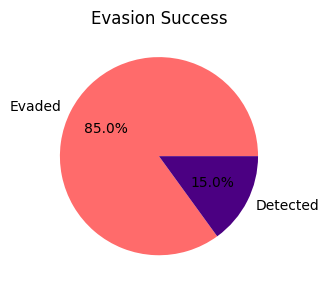
\includegraphics[width=0.6\linewidth]{ evasion_chart.png }
\caption{Evasion success distribution by category}
\end{figure}


\vspace{0.3cm}
\textbf{Actions skipped or delayed by Evasion AI:} \\
\begin{itemize}
    
        
            \item Privilege escalation attempt skipped due to high detection risk
        
    
\end{itemize}

\newpage


% Attack Simulation Summary
\section*{Attack Simulation Summary}

\textbf{Purpose:} This section summarizes the actions executed by the simulated malware, including their outcomes and prioritization. It provides an overview of what was attempted, what succeeded or failed, and how the AI prioritized each action.

\vspace{0.3cm}
\textbf{Actions Executed:} The table below lists all simulated attack actions performed by the Red Team AI Malware Simulator. Each action includes a description, the outcome, and its priority or importance score as determined by the Recon Prioritization AI.

\begin{longtable}{|p{4cm}|p{6cm}|p{2cm}|p{2cm}|}
\hline
\textbf{Action Name} & \textbf{Description} & \textbf{Outcome} & \textbf{Priority / Score} \\
\hline

    
Dummy File Exfiltration & Simulated exfiltration of non-critical test files. & Success & 9 \\
\hline
    
Privilege Escalation & Attempted local privilege escalation (simulated). & Skipped & 8 \\
\hline
    

\end{longtable}

\newpage


% LLM Based Mitigations
\section*{LLM Based Mitigations}

\textbf{Purpose:} This section uses a pre-trained Large Language Model (LLM) to analyze the collected simulation data and generate recommended mitigations for the findings. It provides a concise “briefing for action” rather than a deep technical manual.

\vspace{0.3cm}
\textbf{Note on LLM Limitations:}  
\begin{itemize}
    \item Recommendations are based solely on the simulation data provided.
    \item The LLM may not capture every nuance of real-world system configurations or risks.
    \item Human verification and contextual analysis are recommended before applying any mitigations.
\end{itemize}

\vspace{0.3cm}
\textbf{Recommended Mitigations:}
\begin{itemize}

    
    \item Restrict public file permissions
    
    \item Update outdated software
    
    \item Monitor for suspicious outbound connections
    

\end{itemize}

\newpage


% Raw Data
\section*{Raw Data}
\begin{verbatim}
{
  "sim_start": "2025-10-11 14:00",
  "sim_end": "2025-10-11 16:30",
  "recon_data": {
    "os_name": "Ubuntu",
    "os_version": "22.04.1 LTS",
    "architecture": "64bit",
    "hostname": "test-server",
    "current_user": "root",
    "is_admin": true,
    "open_ports": [
      21,
      80,
      631
    ],
    "env_vars": {
      "PATH": "/usr/bin:/bin",
      "SHELL": "/bin/bash"
    }
  },
  "exec_summary": {
    "open_ports_list": [
      "21 (FTP)",
      "22 (SSH)",
      "80 (HTTP)"
    ],
    "sensitive_data_list": [
      "/home/test/secret.txt",
      "/home/test/passwords.xlsx"
    ],
    "av_list": [
      "ClamAV"
    ],
    "evasion_success": 85,
    "evasion_ai": 85,
    "recon_ai": 90,
    "attack_ai": 75,
    "overall_risk": "Medium"
  },
  "scope": {
    "techniques": "Recon, evasion, dummy file exfiltration, simulated lateral movement."
  },
  "findings": [
    {
      "name": "Open SSH Port",
      "evidence": "Port 22 open on host; SSH service detected (OpenSSH 7.x).",
      "severity": "High",
      "impact": "Could allow remote exploitation if credentials are weak."
    },
    {
      "name": "Sensitive Files in Public Directory",
      "evidence": "/home/test/public/FinancialData.xlsx found.",
      "severity": "Critical",
      "impact": "Confidential data exposure."
    }
  ],
  "evasion": {
    "overall_success": 85,
    "skipped": [
      "Privilege escalation attempt skipped due to high detection risk"
    ],
    "chart_data": [
      {
        "label": "Evaded",
        "value": 85
      },
      {
        "label": "Detected",
        "value": 15
      }
    ]
  },
  "attacks": [
    {
      "name": "Dummy File Exfiltration",
      "description": "Simulated exfiltration of non-critical test files.",
      "outcome": "Success",
      "priority": 9
    },
    {
      "name": "Privilege Escalation",
      "description": "Attempted local privilege escalation (simulated).",
      "outcome": "Skipped",
      "priority": 8
    }
  ],
  "mitigations": [
    "Restrict public file permissions",
    "Update outdated software",
    "Monitor for suspicious outbound connections"
  ]
}
\end{verbatim}

\end{document}